\documentclass[12pt,a4paper,oneside]{ctexart}
\usepackage{amsmath, amsthm, amssymb, graphicx, float}

%导言区
\title{课程《电路与电子学》笔记}
\author{NH5}
\date{更新于2025.3.29}

\begin{document}
\maketitle
\section{直流电路}
电路有两个作用:电能的传递和转换,信号的传递与处理

电路一般由三部分组成:电源、中间环节(如导线、开关)、负载(如电灯、电动机)

\subsection{电路变量}
\subsubsection{电流}
电流:电荷有规则运动形成电流

电流强度:电场作用下,单位时间内通过导体某一横截面的电量.
直流电流用$I=\frac{Q}{t}$表示,时变电流用$i=\frac{dq}{dt}$表示

电流的实际方向:正电荷运动的方向

电流的参考方向:任意假定的电流方向

二者一致电流正值,相反则负值

\subsubsection{电压}
电压:电场力对单位正电荷做功,正电荷从a运动到b,称电场力在这个过程里做的功为这两点之间的电压
用直流电压$U_{ab}=\frac{W_{ab}}{Q}$或时变电压$u_{ab}=\frac{dw_{ab}}{dq}$

类似的,电压实际方向规定为电压从高至低的下降方向,正负值也同电流类似

特殊的,电流的参考方向可以通过下标直接体现:$U_{ab}$表示参考方向为a到b

\subsubsection{关联参考方向}
电压电流的方向均可任意取定,所以存在二者相同或相反的情况,
规定二者一致时称为\textbf{关联参考方向},
不一致则为\textbf{非关联参考方向}.
推荐使用关联参考方向

\subsubsection{电位}
在一个电路中,选取某一个点作为参考点,规定参考点的点位为0,由于任意两点之间的电压等于这两点的电位差,
这样就可以得到电路中任意一点的电位以及任意两点之间的电压

在一个电路中,参考点有且只有一个点

改变参考点,可能会改变某一点的电位值,但是不会改变两点之间的电压值

\subsubsection{功率和能量}
电功率:单位时间内元件吸收或发出的电能,$p=\frac{dW}{dt}=\frac{dW}{dq}\frac{dq}{dt}=ui$

如果$p>0$则称元件吸收功率(负载),反之则是元件提供功率(电源)

\subsection{电阻元件}
欧姆定律:$R=\frac{u}{i}$

电导:$G=\frac{1}{R}$,单位:西门子(S)

电阻的功率:$p=\frac{u^2}{R}=Ri^2$

\subsection{电压源与电流源}
\subsubsection{理想源}
理想电压源:电压恒定,电流任意

理想电流源:电流恒定,电压任意

\subsubsection{短路和断路}
短路:电压为零,相当于导线

断路:又称开路,电流为零

\subsubsection{实际电压源}
可以视为理想电压源$U_S$与电阻$R_S$串联形成的整体

其伏安特性可表示为$U=U_S-IR_S$,
则有开路电压$U_{OC}=U_S$,短路电流$I_{SC}=\frac{U_S}{R_S}$

\subsubsection{实际电流源}
可以视为理想电流源$I_S$与电阻$R_S$并联形成的整体

其伏安特性可表示为$I=I_S-\frac{U}{R_S}$,
则有开路电压$U_{OC}=R_SI_S$,短路电流$I_{SC}=I_S$

\subsection{基尔霍夫定律}
\subsubsection{基本概念}
支路:电路中的每一个分支

节点:三条或以上支路的连接点

回路:由支路组成的闭合路径

网孔:内部不含任何支路的回路
\begin{figure}[H]
    \centering
    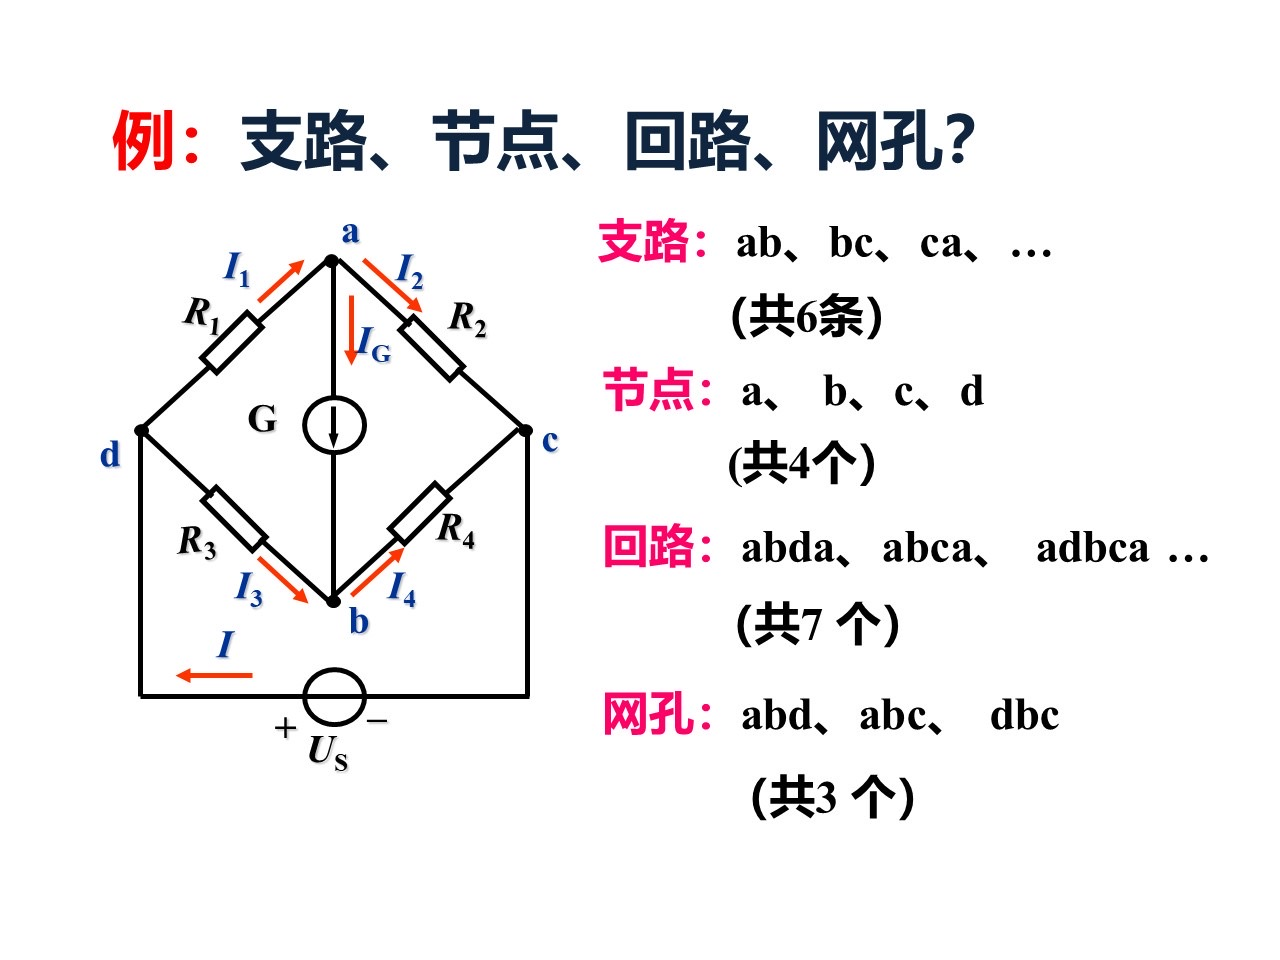
\includegraphics[width=8cm]{photos/支路节点回路网孔.jpg}
\end{figure}

\subsubsection{KCL}
基尔霍夫电流定律(KCL):对于任意时刻的任一节点,流出的电流代数和为0

另一种表述:对于任意时刻的任一节点,流入电流和等于流出电流和

KCL可以推广至任一假设的闭合面,称为广义节点

\subsubsection{KVL}
基尔霍夫电压定律(KVL):沿任一闭合回路绕行一周,各支路的电压代数和为零

\subsection{支路电流分析法}
支路电流法:以支路电流为未知量,应用(KCL,KVL)列方程求解.

\textbf{先列KCL方程}:对每个节点列出KCL方程$\bf{CI}=\bf{0}$,矩阵$\bf{C}$不是行满秩矩阵,
所以需要从原始方程组中去掉某些方程保证系数矩阵行满秩.由于一个方程对应电路中一个节点.
所以称保留的节点为独立节点,一般去除一个方程就行,所以称去除的节点为参考节点.

\textbf{再列KVL方程}:同KCL方程一样,我们要保证方程的独立,所以我们在选取回路时要保证下一个回路中有前几个回路中未出现的回路.
独立回路方程选择不唯一,一般优先考虑网孔.

\subsection{叠加定理}
叠加定理:在电路中,考察某一支路的电压(或电流),可以先分别考虑各个源对这个支路的作用,再线性叠加.
叠加原理不能用于功率等的分析,因为功率不是线性的.

\subsection{含受控源的电阻电路}
为了分析与计算方便,把电路分成三个部分:电源,中间环节,负载.
\begin{figure}[H]
    \centering
    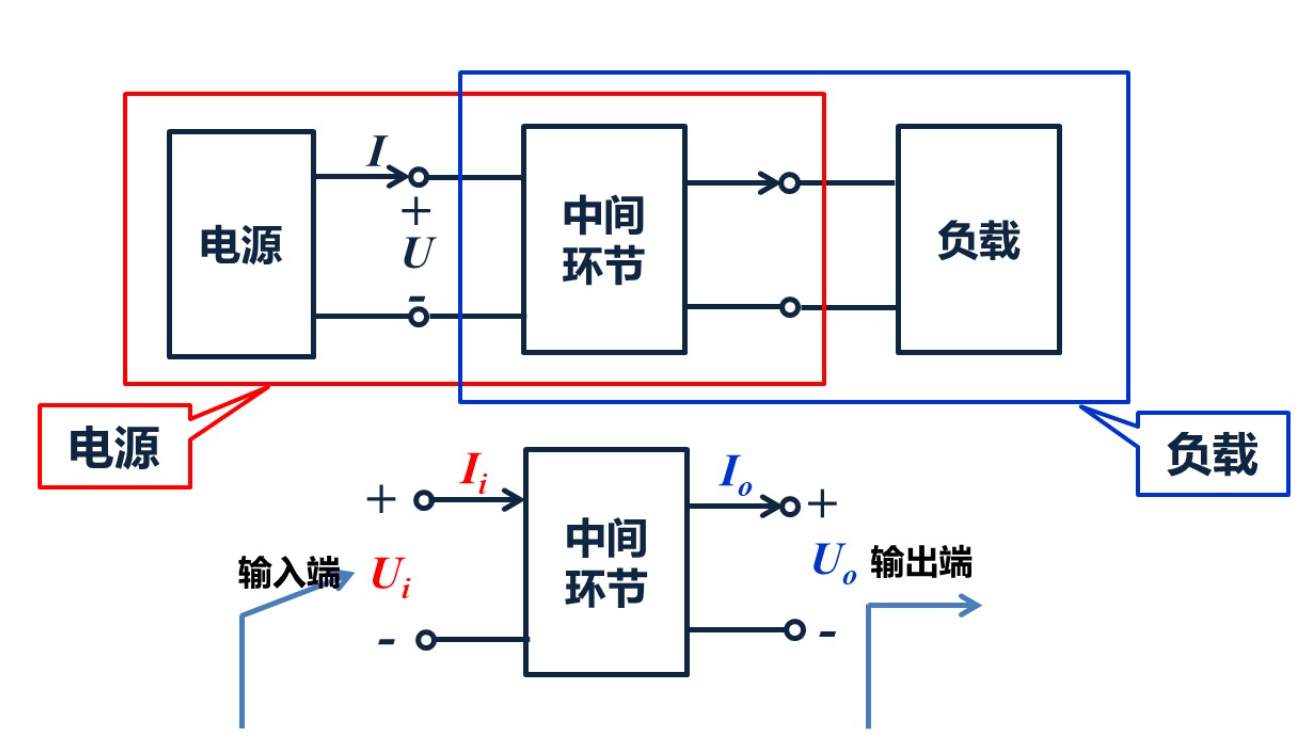
\includegraphics[width=8cm]{photos/双口网络.png}
\end{figure}

中间环节就是一个双口网络:具有两个外接端口的电路,又称二端口网络

输入端有$I_i$和$U_i$,输出端有$I_0$和$U_0$

\subsubsection{戴维南定理}
任意一个线性有源单口网络,就其对外电路的作用而言,总可以用一个理想电压源和一个电阻串联的支路来等效

理想电压源的电压等于有源线性单口网络的开路电压$U_{oc}$,串联电阻$R_o$等于该网络中所有独立电源置零时的等效电阻

\subsubsection{诺顿定理}
任意一个有源线性单口网络,就其对外电路的作用而言,总可以用一个理想电流源和一个电阻并联来等效

其中电流源的电流等于有源线性单口网络的短路电流$I_{se}$,并联电阻$R_o$等于将此网络中所有独立电源置零后的等效电阻

实际上,戴维南电路与诺顿电路是等效的

\subsubsection{受控电源}
前面讲的电压源和电流源都是独立电源,这种电压源的电压和电流源的电流是不受外电路控制而独立存在的.
然而电子电路中往往还有另外一种类型的电源,它的电压源的电压和电流源的电流受到同一电路中其他支路的电压或电流控制,
这种电源称为受控源.为与独立源区别,受控源用菱形符号表示.

以下是四种受控源模型:
\begin{figure}[H]
    \centering
    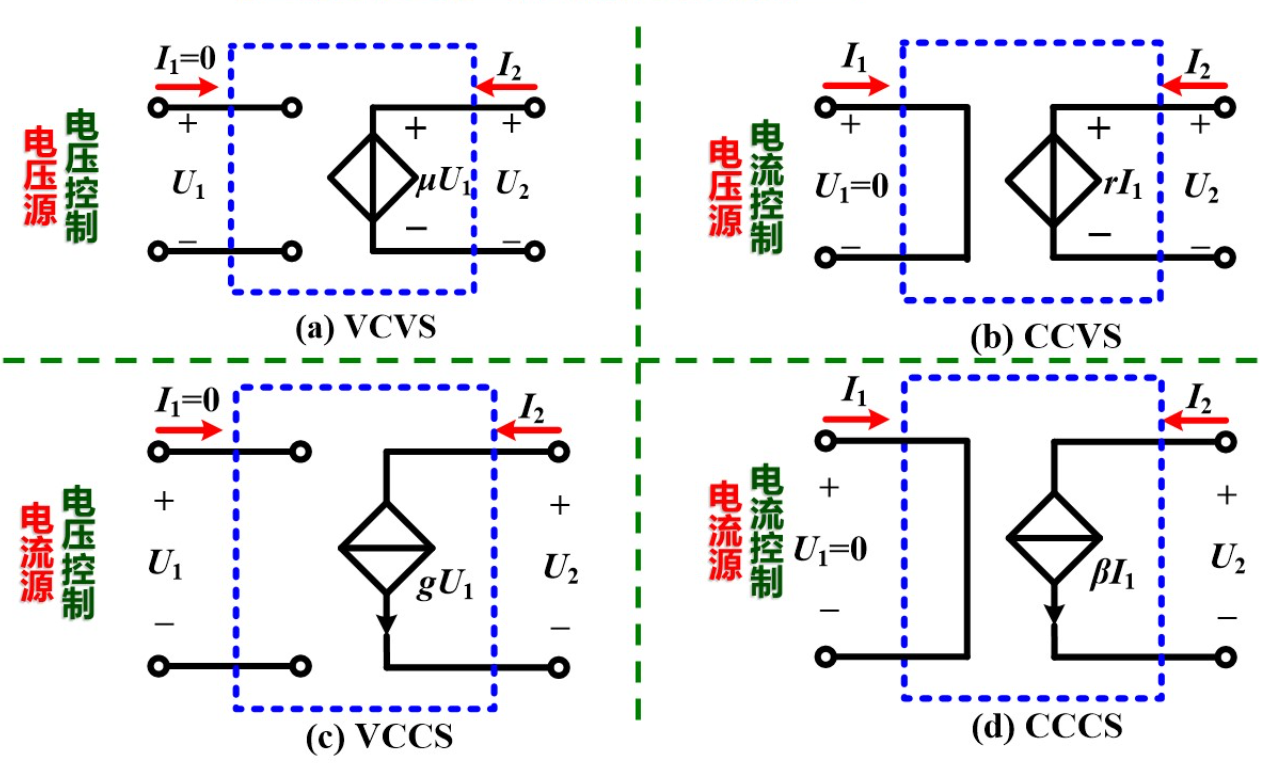
\includegraphics[width=8cm]{photos/四种受控源模型.png}
\end{figure}

当电路中含受控源时,仍可采用前面介绍的支路电流法,节点电压法,叠加原理,戴维南定理等进行分析,
但要注意以下几点:

1.化简电路时,当受控源还被保留时,不要把受控源的控制量消除

2.在应用支路电流法和节点电位法时,可以把受控源看作电压源或电流源

3.应用叠加原理或等效电源时,应保留受控源,不能像独立源那样处理

4.使用叠加原理时,受控源的控制量随着不同独立源的作用而变化
\end{document}